\section{Designing SimpleSpeech}
Building on the capabilities developed in these prior studies, SimpleSpeech is a web-based application for recording and editing short voice messages in a discussion setting.
Our user interface is quite similar to those created by Rubin \cite{rubin}, Yoon \cite{yoon}, and Whittaker \cite{whittaker_semantic}, which also provide lightweight audio editing capabilities.
Nevertheless, some slight conceptual modifications were necessary to suit the ``live'' editing paradigm, which we discuss below.
The appearance of the final SimpleSpeech user interface (UI) is shown in Fig. \ref{fig:overview_shot}.

Our text-based approach to speech editing requires a reliable transcription as well as time intervals corresponding to each word.
Both of these requirements are fulfilled by the IBM Watson Developer Cloud speech-to-text transcription service, which is reported to have a word error rate of 10.4\% \cite{soltau:2014}.

We chose to include a waveform visualization as part of the UI in order to remind the user that he or she is ultimately manipulating audio, not text. 
The waveform incorporates several subtle indications of the mapping between its contents and the transcription, including highlighting the audio corresponding to the current selection of tokens and animating deletions and insertions.
We found the presence of a waveform to be a helpful visual indicator of the purpose of SimpleSpeech because without it, users' inclination was to disregard the original speech and use the system as a dictation tool.

Our use of text as a proxy for editing audio rendered it necessary to clearly delineate the capabilities of SimpleSpeech in comparison to a word processor.
However, we found the capability to edit text of individual words in the transcript to be desirable, especially in the case of ASR errors.
As shown in Fig. \ref{fig:transcription}, the transcription editing functionality is available in a separate mode, accessed by pressing the Return key.
The pop-up box insulates the editing within single words to avoid undermining the cohesiveness of the tokens. 

\begin{figure}
	\centering
	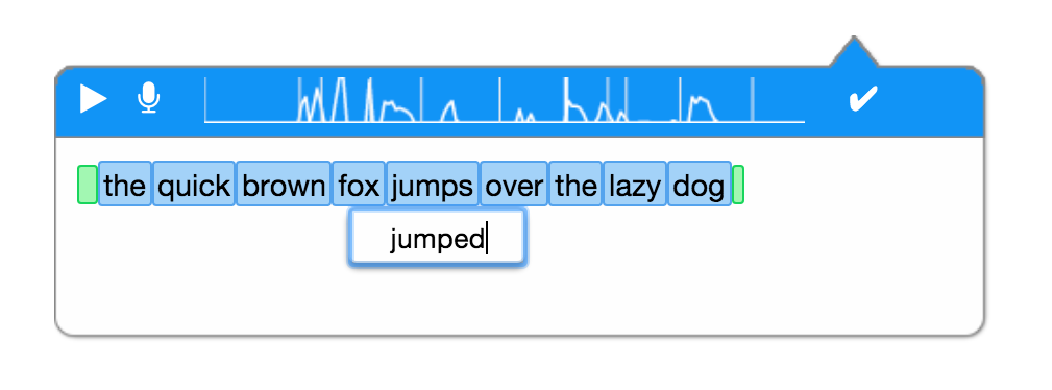
\includegraphics[width=\columnwidth,keepaspectratio]{figures/transcription_edit}
	\caption{To keep the user interface from becoming cluttered with secondary functionality, the transcription editing feature was implemented as a modal interaction. The pop-up box shown above ``opens'' the selected tokens for text editing in a separate control element, thus notifying the user that he or she is no longer directly editing the audio.}
	\label{fig:transcription}
\end{figure}

\subsection{Pilot Study and Design Improvements}
We followed an iterative procedure to progressively improve the design and interactions of SimpleSpeech.
After building an initial prototype of the application, an informal pilot test was conducted with 5 participants (4 female, 1 male). 
Each user was given a brief introduction to the software and shown how to use the basic features, then given the scenario of creating an audio response to a written claim on an online forum. 
(The prompts used in the tests were adapted from the GRE Pool of Issue Topics.)
After using the software, users were interviewed to obtain feedback on the prototype, yielding the following modifications:

\begin{itemize}
\item a Shift+space shortcut for controlling playback, which constitutes a \emph{quasi-mode} accessed by pressing the Shift key; and
\item the ability to introduce and adjust pauses between words, not just to remove them.
\end{itemize}